\subsection{Loadtest}
Bei den Loadtests werden nur die Ergebnisse der Szenarien unter "Average Load" im Einzelnen vorgestellt.
Dabei werden auch die wichtigsten Messwerte zur Bestimmung der Zuverlässigkeit aggregiert aus allen Testdurchführungen angezeigt.
„CPU Max” und „Memory Max” zeigen, wie viel die Anwendung maximal an RAM und CPU während der Tests verbraucht hat.
„Node CPU MAX” und „Node Memory MAX” zeigen, wie viel das gesamte System maximal an RAM und CPU verbraucht hat. Bei Docker Compose wäre dies eine VM, während es bei k3s der gesamte Cluster wäre.
Beide Werte sind jeweils normiert, um die Umgebungen fairer vergleichen zu können.
Die Error Rate zeigt, wie viele HTTP-Anfragen fehlgeschlagen sind.
Es wird auch angezeigt, wie viele Restarts von Containern in Docker Compose und wie viele Pods in der K3s-Umgebung in allen Testdurchläufen zusammengezählt wurden.

Bei jedem Szenario wird auch die Auswertung für jeden Testdurchlauf angezeigt, der mit „Average Load” lief, sowie das aggregierte Scoring aller Testumgebungen.
Zum Schluss jedes Szenarios wird die durchschnittliche Zuverlässigkeit jeder Testmethode angezeigt.
\subsubsection{Login}
Wie in Abbildung \ref{fig:login_reliability_score} zu sehen ist, hat jeder Testdurchlauf beim Average Load Test vom Login ein Scoring von über 60 von 100 Punkten erreicht.
Dabei konnte die k3s-Umgebung jedes Mal ein höheres Scoring als die Docker-Compose-Umgebung erzielen.

Interessant ist der höhere maximale CPU-Verbrauch der Anwendung in der Docker-Compose-Umgebung im Vergleich zur k3s-Umgebung, wie in Tabelle \ref{tab:login_average_load_metrics} zu sehen ist.
Während der maximale CPU-Verbrauch des gesamten Systems in beiden Umgebungen näher beieinander liegt. Dabei erreicht die Node-CPU-Max aber eine Auslastung von über 100 \%.
\begin{table}[htbp]
\centering
\caption{Vergleich der Durchschnittswerte aller Test zur bestimmung der Zuverlässigkeit für das Login-Szenario unter Average Load}
\label{tab:login_average_load_metrics}

\begin{tabular}{lrr}
\toprule
\textbf{Metrik} & \textbf{Docker} & \textbf{K3s} \\
\midrule
Error Rate [\%]        & 0.0000 & 0.0008 \\
CPU Max [\%]           & 99.45  & 33.47 \\
Memory Max [\%]        & 46.07  & 12.56 \\
Node CPU Max [\%]      & 99.98  & 104.96 \\
Node Memory Max [\%]   & 51.00  & 70.79 \\
Restarts               & 0.00   & 0.00 \\
\bottomrule
\end{tabular}

\end{table}

\begin{figure}[htbp]
\centering
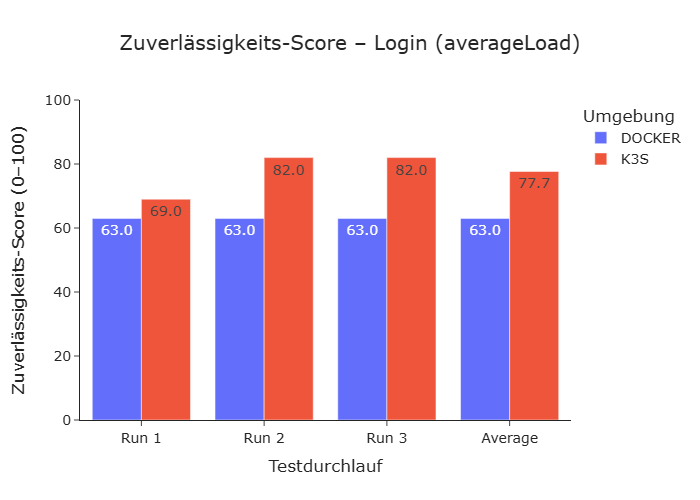
\includegraphics[width=0.8\textwidth]{bilder/tests/reliability_score_login_averageLoad.png}
\caption{Reliability Score für das Login-Szenario unter Average Load}
\label{fig:login_reliability_score}
\end{figure}

Vergleichen wir nun die durchschnittliche Zuverlässigkeit der Score-Werte jedes Tests des Login-Szenarios, die in der Tabelle \ref{tab:scenario_score_matrix_login} zu sehen ist, so zeigt sich, dass die k3s-Umgebung bei jedem Test die bessere Zuverlässigkeit erreicht, bis auf den Smoke-Test bei dem beide die Maximalpunktzahl erreichen konnten.
Bis auf den Spike-Test bleiben beide Umgebungen nah beieinander.

\begin{table}[htbp]
\centering
\caption{Durchschnittlicher Reliability Score pro Testtyp für das Szenario Login}
\label{tab:scenario_score_matrix_login}

\begin{tabular}{lccccc}
\toprule
\textbf{Environment} & \textbf{Smoke} & \textbf{Average Load} & \textbf{Stress} & \textbf{Spike} & \textbf{Breaking Point} \\
\midrule
Docker & 100.00 & 63.00 & 59.67 & 38.00 & 53.00 \\
K3s    & 100.00 & 77.67 & 65.00 & 60.00 & 65.00 \\
\bottomrule
\end{tabular}

\end{table}

\FloatBarrier
\subsubsection{Vorlesungen}
Wie in Abbildung \ref{fig:vorlesungen_reliability_score} zu sehen ist, hat bei den Vorlesungen unter Average Load kein Testdurchlauf einen Score über 50 von 100 Punkten erreicht.
Die k3s-Umgebung hat dabei wieder einen höheren Score als die Docker-Compose-Umgebung erhalten.
In den in Tabelle \ref{tab:vorlesungen_average_load_metrics} aufgeführten Messwerten ist besonders interessant, dass beide Umgebungen eine hohe Fehlerrate für eine Webanwendung aufweisen.
Dabei hat die k3s-Umgebung fast doppelt so viele Fehler wie die Docker-Compose-Umgebung.
Trotz der niedrigeren Fehlerrate hat die Anwendung in der Docker-Compose-Umgebung einen höheren CPU- und RAM-Verbrauch als die k3s-Umgebung.
\begin{table}[htbp]
\centering
\caption{Vergleich der Durchschnittswerte aller Test zur bestimmung der Zuverlässigkeit für das Vorlesungen-Szenario unter Average Load}
\label{tab:vorlesungen_average_load_metrics}

\begin{tabular}{lrr}
\toprule
\textbf{Metrik} & \textbf{Docker} & \textbf{K3s} \\
\midrule
Error Rate [\%]        & 2.38 & 4.65 \\
CPU Max [\%]           & 99.57 & 44.18 \\
Memory Max [\%]        & 74.66 & 23.58 \\
Node CPU Max [\%]      & 99.98 & 109.63 \\
Node Memory Max [\%]   & 81.25 & 81.02 \\
Restarts               & 0.00 & 0.00 \\
\bottomrule
\end{tabular}

\end{table}

\begin{figure}[htbp]
\centering
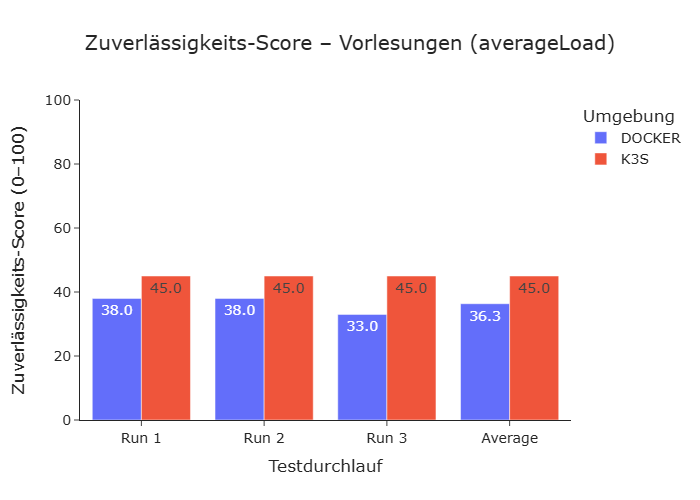
\includegraphics[width=0.8\textwidth]{bilder/tests/reliability_score_vorlesungen_averageLoad.png}
\caption{Reliability Score für das Vorlesungen-Szenario unter Average Load}
\label{fig:vorlesungen_reliability_score}
\end{figure}

Ein Vergleich der durchschnittlichen Zuverlässigkeitsscores jeder Testmethode in dem Szenario „Vorlesungen“, wie in Tabelle \ref{tab:scenario_score_matrix_vorlesungen} dargestellt, zeigt, dass die Docker-Compose-Umgebung in den meisten Testmethoden einen höheren Score erreichen konnte.
Nur beim „Average Load” konnte die „k3s”-Umgebung einen höheren Score als die „Docker Compose”-Umgebung erzielen. 
Bei „Smoke” haben beide Umgebungen wieder den gleichen Score erzielt.
Die Abstände zwischen den Umgebungen sind jeweils nicht allzu groß.

\begin{table}[htbp]
\centering
\caption{Durchschnittlicher Reliability Score pro Testtyp für das Szenario Vorlesungen}
\label{tab:scenario_score_matrix_vorlesungen}

\begin{tabular}{lccccc}
\toprule
\textbf{Environment} & \textbf{Smoke} & \textbf{Average Load} & \textbf{Stress} & \textbf{Spike} & \textbf{Breaking Point} \\
\midrule
Docker & 75.00 & 36.33 & 38.00 & 38.00 & 38.00 \\
K3s    & 75.00 & 45.00 & 31.67 & 25.00 & 25.00 \\
\bottomrule
\end{tabular}

\end{table}

\FloatBarrier
\subsubsection{Klausur}
Wie in Abbildung \ref{fig:klausur_reliability_score} zu sehen ist, blieb der Score bei den Klausuren unter Average Load bei jedem Testdurchlauf unter 20 von 100 Punkten.
Im zweiten Testdurchlauf gab es einen Ausschlag der k3s-Umgebung, in der ein Score von 0 Punkten erreicht wurde.
In den übrigen Testdurchläufen konnte die k3s-Umgebung einen besseren Score erzielen, blieb aber jedes Mal unter dem Score der Docker-Compose-Umgebung.
Dabei kann in Tabelle \ref{tab:klausur_average_load_metrics} erneut eine hohe Fehlerrate festgestellt werden, wobei diese in der Docker-Compose-Umgebung mehr als die Hälfte kleiner ist als in der k3s-Umgebung.
Die Anwendung in der Docker-Compose-Umgebung verbraucht aber wieder deutlich mehr CPU als in der k3s-Umgebung.
Auffällig ist auch, dass die k3s-Umgebung achtmal Pods neustarten musste.

\begin{table}[htbp]
\centering
\caption{Vergleich der Durchschnittswerte aller Test zur bestimmung der Zuverlässigkeit für das Klausur-Szenario unter Average Load}
\label{tab:klausur_average_load_metrics}

\begin{tabular}{lrr}
\toprule
\textbf{Metrik} & \textbf{Docker} & \textbf{K3s} \\
\midrule
Error Rate [\%]        & 5.43 & 12.05 \\
CPU Max [\%]           & 99.64 & 27.91 \\
Memory Max [\%]        & 63.12 & 19.80 \\
Node CPU Max [\%]      & 99.67 & 101.98 \\
Node Memory Max [\%]   & 66.95 & 78.60 \\
Restarts               & 0.00 & 8.00 \\
\bottomrule
\end{tabular}

\end{table}

\begin{figure}[htbp]
\centering
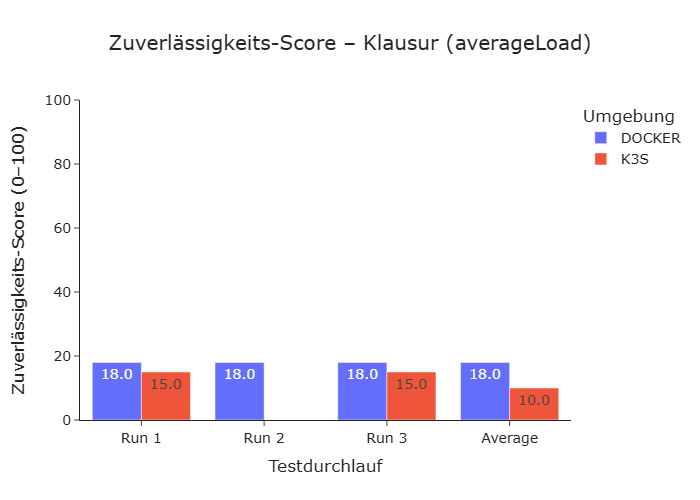
\includegraphics[width=0.8\textwidth]{bilder/tests/reliability_score_klausur_averageLoad.png}
\caption{Reliability Score für das Klausur-Szenario unter Average Load}
\label{fig:klausur_reliability_score}
\end{figure}

Beim Vergleich der durchschnittlichen Zuverlässigkeitswerte jeder Testmethode im Szenario „Klausur“, die in der Tabelle \ref{tab:scenario_score_matrix_klausur} zu sehen ist, fällt auf, dass die Docker-Compose-Umgebung wieder fast immer einen höheren Score als die k3s-Umgebung erzielt hat, bis auf den Spike-Test.
Dennoch bleibt festzuhalten, dass sich die Umgebungen nicht zu stark unterscheiden.
\begin{table}[htbp]
\centering
\caption{Durchschnittlicher Reliability Score pro Testtyp für das Szenario Klausur}
\label{tab:scenario_score_matrix_klausur}

\begin{tabular}{lccccc}
\toprule
\textbf{Environment} & \textbf{Smoke} & \textbf{Average Load} & \textbf{Stress} & \textbf{Spike} & \textbf{Breaking Point} \\
\midrule
Docker & 55.00 & 18.00 & 18.00 & 18.00 & 18.00 \\
K3s    & 41.33 & 10.00 & 17.00 & 23.00 & 6.67 \\
\bottomrule
\end{tabular}

\end{table}
\FloatBarrier